\section{Algoritmos de clasificación}
Se han utilizado diversos algoritmos de aprendizaje automático para la clasificación de textos, dentro de los más populares y frecuentemente utilizados como línea base son las máquinas de soporte vectorial o SVM por sus siglas en inglés. Por otro lado, respecto a las arquitecturas de aprendizaje profundo que se han empezado a emplear, se distinguen dos arquitecturas básicas: las redes recurrentes y las redes convoluciones. En esta sección se explican las generalidades de estos algoritmos. En \citep{Minaee2020} se puede encontrar una revisión más detallada del estado del arte en la clasificación de textos con aprendizaje profundo.


\subsection{Máquinas de Soporte Vectorial (SVM)}
Este algoritmo de clasificación fue propuesto por \citep{vapnik1964class}, desde entonces el algoritmo ha pasado por una serie de mejoras. \citep{boser1992training} adaptó el algoritmo para resolver problemas no lineales  y la formulación moderna fue desarrollada por \citep{cortes1995support}.

Retomando las definiciones de \citep{boser1992training}, SVM encuentra una función de decisión para vectores $x$ de características de dimensión $n$ pertenecientes a alguna clase A o B. La entrada al algoritmo de entrenamiento es un conjunto de $p$ ejemplos $x_i$ con etiquetas $y_i$:

\begin{equation} \label{eq:training}
(x_1, y_1), (x_2, y_2), (x_3, y_3), ... , (x_p, y_p) 
\end{equation}

\[
    \text{donde}
    \begin{cases}
        y_k=1 & \text{si $x_k \in A$}\\
        y_k=-1 & \text{si $x_k \in B$}
    \end{cases}
\]

Para los ejemplos de entrenamiento el algoritmo encuentra una función de decisión $D(x)$ durante una fase de aprendizaje. Después del entrenamiento, la clasificación de patrones desconocidos es predicha de acuerdo a la siguiente regla:

\begin{equation} \label{eq:svm_de}
\begin{split}
    x \in A \text{ si } D(x)>0 \\
    x \in B \text{ si no } 
\end{split}
\end{equation}

Las funciones de decisión deben ser lineales en sus parámetros pero no están restringidas a dependencias lineales de $x$. Estas funciones pueden ser expresadas idénticamente a un \textit{perceptron }\citep{block1962analysis}:

\begin{equation} \label{eq:percetron}
    D(x) = \sum_{i=1}^{N} w_i\phi_i(x) + b
\end{equation}

En la ecuación \ref{eq:percetron} $ \phi_i$ son funciones predefinidas de $x$ y $w_i$ y $b$ son los parámetros ajustables a aprender.

En la formulación de \citep{boser1992training, cortes1995support} podemos encontrar como aproximar este tipo de funciones construyendo hiperplanos separados que maximicen un margen, mediante algoritmos de optimización numérica. \\

Las ventajas\footnote{Listadas en https://scikit-learn.org/stable/modules/svm.html} de SVM son: 
\begin{itemize}
    \item Son efectivas en espacios altamente dimensionales, como es el caso en la clasificación de textos.
    \item Son efectivas en casos en donde el número de dimensiones es mayor al número de ejemplos.
    \item Usa un subconjunto de puntos de entrenamiento en la función de decisión llamados vectores de soporte, así que es también eficiente en el uso de la memoria.
    \item Se pueden especificar diferentes funciones de núcleo para la función de decisión. 
\end{itemize}

Las desventajas incluyen:
\begin{itemize}
    \item Si el número de características es mucho mayor al número de ejemplos, elegir una función de núcleo y término de regularización es crucial para evitar el sobre ajuste.
    \item Las SVMs no otorgan directamente estimaciones de probabilidad, éstas son calculadas utilizando validación cruzada.
    
\end{itemize}
    
    
    
%\subsubsection{C-SVM}

\subsection{Redes neuronales profundas}

En la definición de \citep{lecun2015deep}, el aprendizaje profundo permite a los modelos computaciones que están compuestos de múltiples capas de procesamiento aprender representaciones de los datos con múltiples niveles de abstracción. Estos métodos han mejorado dramáticamente el estado del arte en el varias tareas en el entendimiento de lenguaje natural, particularmente, clasificación de textos, análisis de sentimientos, respuesta a preguntas y traducción automática. El aprendizaje profundo descubre estructuras en grandes conjuntos de datos utilizando el algoritmo de retro-propagación para determinar sus parámetros internos que son utilizados para calcular la representación en cada capa de la arquitectura.

A continuación se describen los conceptos principales en aprendizaje profundo tomados principalmente de \citep{lecun2015deep}, para una definición mas extensa consultar \citep{kamath2019deep, goodfellow2016deep}.

\subsubsection{Retropropagación y entrenamiento de arquitecturas multicapa}

Una arquitectura multicapa es una pila de modelos simples y muchos de éstos calculan un mapeo entrada-salida no lineal. El procedimiento de retro-propagación que calcula el gradiente de una función objetivo con respecto a los pesos de múltiples capas es una aplicación práctica de la regla de la cadena para derivadas.

Las arquitecturas multicapa aprenden a mapear una entrada de tamaño fijo (por ejemplo, la representación vectorial de un documento) a una salida de tamaño fijo (por ejemplo, las categorías de documentos). Para ir de una capa a la siguiente, un conjunto de unidades (nodos o neuronas) calculan una suma pesada de las entradas de la capa anterior y el resultado es pasado a través de una función no lineal. A la fecha, la función ReLU (\ref{eq:RELU})  es una de las más populares ya que se ha demostrado empíricamente que permite aprender más rápido en redes neuronales con muchas capas \citep{glorot2011deep}. Las neuronas que no forman parte de la capa de entrada ni la de salida se conocen como unidades ocultas. 

Las\textbf{ capas ocultas} pueden ser vistas como una distorsión de la entrada en una forma no lineal para que las categorías sean linealmente separables por la última capa.

\begin{equation} \label{eq:RELU}
    f(z)= max(z,0)
\end{equation}

La \textbf{capa de entrada} puede ser construida vía pesado TF-IDF, vectores de palabras o alguna otra característica o representación. En la clasificación de documentos usualmente la capa de entrada recibe un documento en representación vectorial (\ref{eq:vectorspace}).

\begin{equation} \label{eq:vectorspace}
d_{j} = (w_{1,j},w_{2,j},...,w_{i,j}...,w_{l_{j},j})
\end{equation}

En donde $l_{j}$ es el tamaño del documento $j$, y $w_{i,j}$ es la representación vectorial de la palabra $i$ en el documento $j$.

En la \textbf{capa de salida} el numero de neuronas es igual al número de clases para clasificaciones con más de dos clases y una para clasificación binaria, es la encargada de realizar la predicción final en base a las representaciones capturadas por la red neuronal.

La \textbf{inicialización} de los pesos y sesgo (bias) por lo general es con ceros o números generados con base en algún criterio, un algoritmo común de idealización es el conocido como inicialización Glorot o Xavier \citep{glorot2010understanding}, el cual es basado en números aleatorios extraídos de una distribución de probabilidad uniforme.

Cuando se entrena una red neuronal, la propagación hacia adelante es realizada en lotes o \textbf{batch} (un número de instancias de entrenamiento determinado por el hiper-parámetro llamado tamaño de batch), después se calcula el error para cada neurona mediante retro-propagación en el mismo lote. 

Una \textbf{época} es una sola iteración sobre todo el conjunto de datos, el número de épocas es un hiper-parámetro que determina cuantas veces el algoritmo de aprendizaje itera sobre todo el conjunto de entrenamiento.

%\subsubsection{Regularización}
%L1 , L2, Batch, Augment , Drotout

%\subsubsection{Optimización}
% Adam, cross-entropy, loss 

%Durante la fase de entrenamiento 

%%Agregar algunas imagenes chidas del paper de Lecun 2015


\subsubsection{Redes Neuronales Recurrentes (RNN)}
Los modelos basados en RNNs tienen el objetivo principal de capturar la dependencia entre palabras y la estructura del texto para clasificación de textos \cite{goodfellow2016deep}.

La redes recurrentes procesan una secuencia $u_t$ como entrada, un elemento a la vez, manteniendo en sus neuronas ocultas un  ``vector de estado" $x_t$ que implícitamente contiene información acerca de todos los elementos anteriores a la secuencia procesada \cite{lecun2015deep}. La formulación general de este concepto es presentado en la ecuación \ref{eq:rrn}, en donde $x_t$ es el vector de estado en tiempo $t$ y $u_t$ se refiere a la entrada en el paso $t$.


\begin{equation} \label{eq:rrn}
    x_t = F(x_{t-1}, u_t, \theta )
\end{equation}


Las redes recurrentes son sistemas dinámicos muy poderosos, pero su entrenamiento es muy problemático dado que su gradiente al ser retro-propagado crece o disminuye en cada paso, así que sobre cada paso típicamente explotan o desaparecen \citep{lecun2015deep}, para tratar de solucionar este problema se propuso un tipo especial de red recurrente conocida como LSTM.

\subsubsection{LSTM}
Propuestas originalmente por \citep{hochreiter1997long} para tratar los problemas de explotación y desvanecimiento de gradientes en redes recurrentes, las redes de memoria a corto y largo plazo son un tipo especial de red recurrente que conserva las dependencias largas de maneras más efectivas en comparación con una red recurrente básica. Las redes LSTM usan múltiples capas para regular el monto de información que será permitida en cada estado de nodo. La figura \ref{fig:LSTM} muestra la estructura interna de una celda de una LSTM. En donde $x_t$, $o$ y $h_t$ representan la entrada, salida y el estado oculto en tiempo $t$. $c_{t-1}$ es la información llevada del estado $t-1$ al estado $t$, el cual será combinado con la entrada $x_t$ y el estado oculto $h_{t-1}$ para formar el estado oculto $h_t$ y el arrastre de $c_t$ el cual será enviado al siguiente paso.

\subsubsection{Redes recurrentes bi-direccionales}
Las redes recurrentes convencionales consideran una estructura causal, significando que cada estado en tiempo $t$ captura solo información del pasado, $x,..., x^{t-1}$, y la entrada actual $x^t$. Sin embargo en muchas aplicaciones para realizar una predicción de $y^t$ que dependa de la secuencia entera, las RNNs bidireccionales fueron propuestas para resolver ese problema  \citep{schuster1997bidirectional}. Las RNNs bidireccionales combinan una red recurrente que se mueve hace adelante en el tiempo, comenzando desde el inicio del texto, con otra que se mueve hacia adelante en el tiempo, comenzando desde el fin del texto, para obtener una representación final se combina la red hacia adelante y hacia atrás mediante alguna operación con tensores (suma, concatenación, multiplicación o promedio). 



\begin{figure}[!t]
\centering
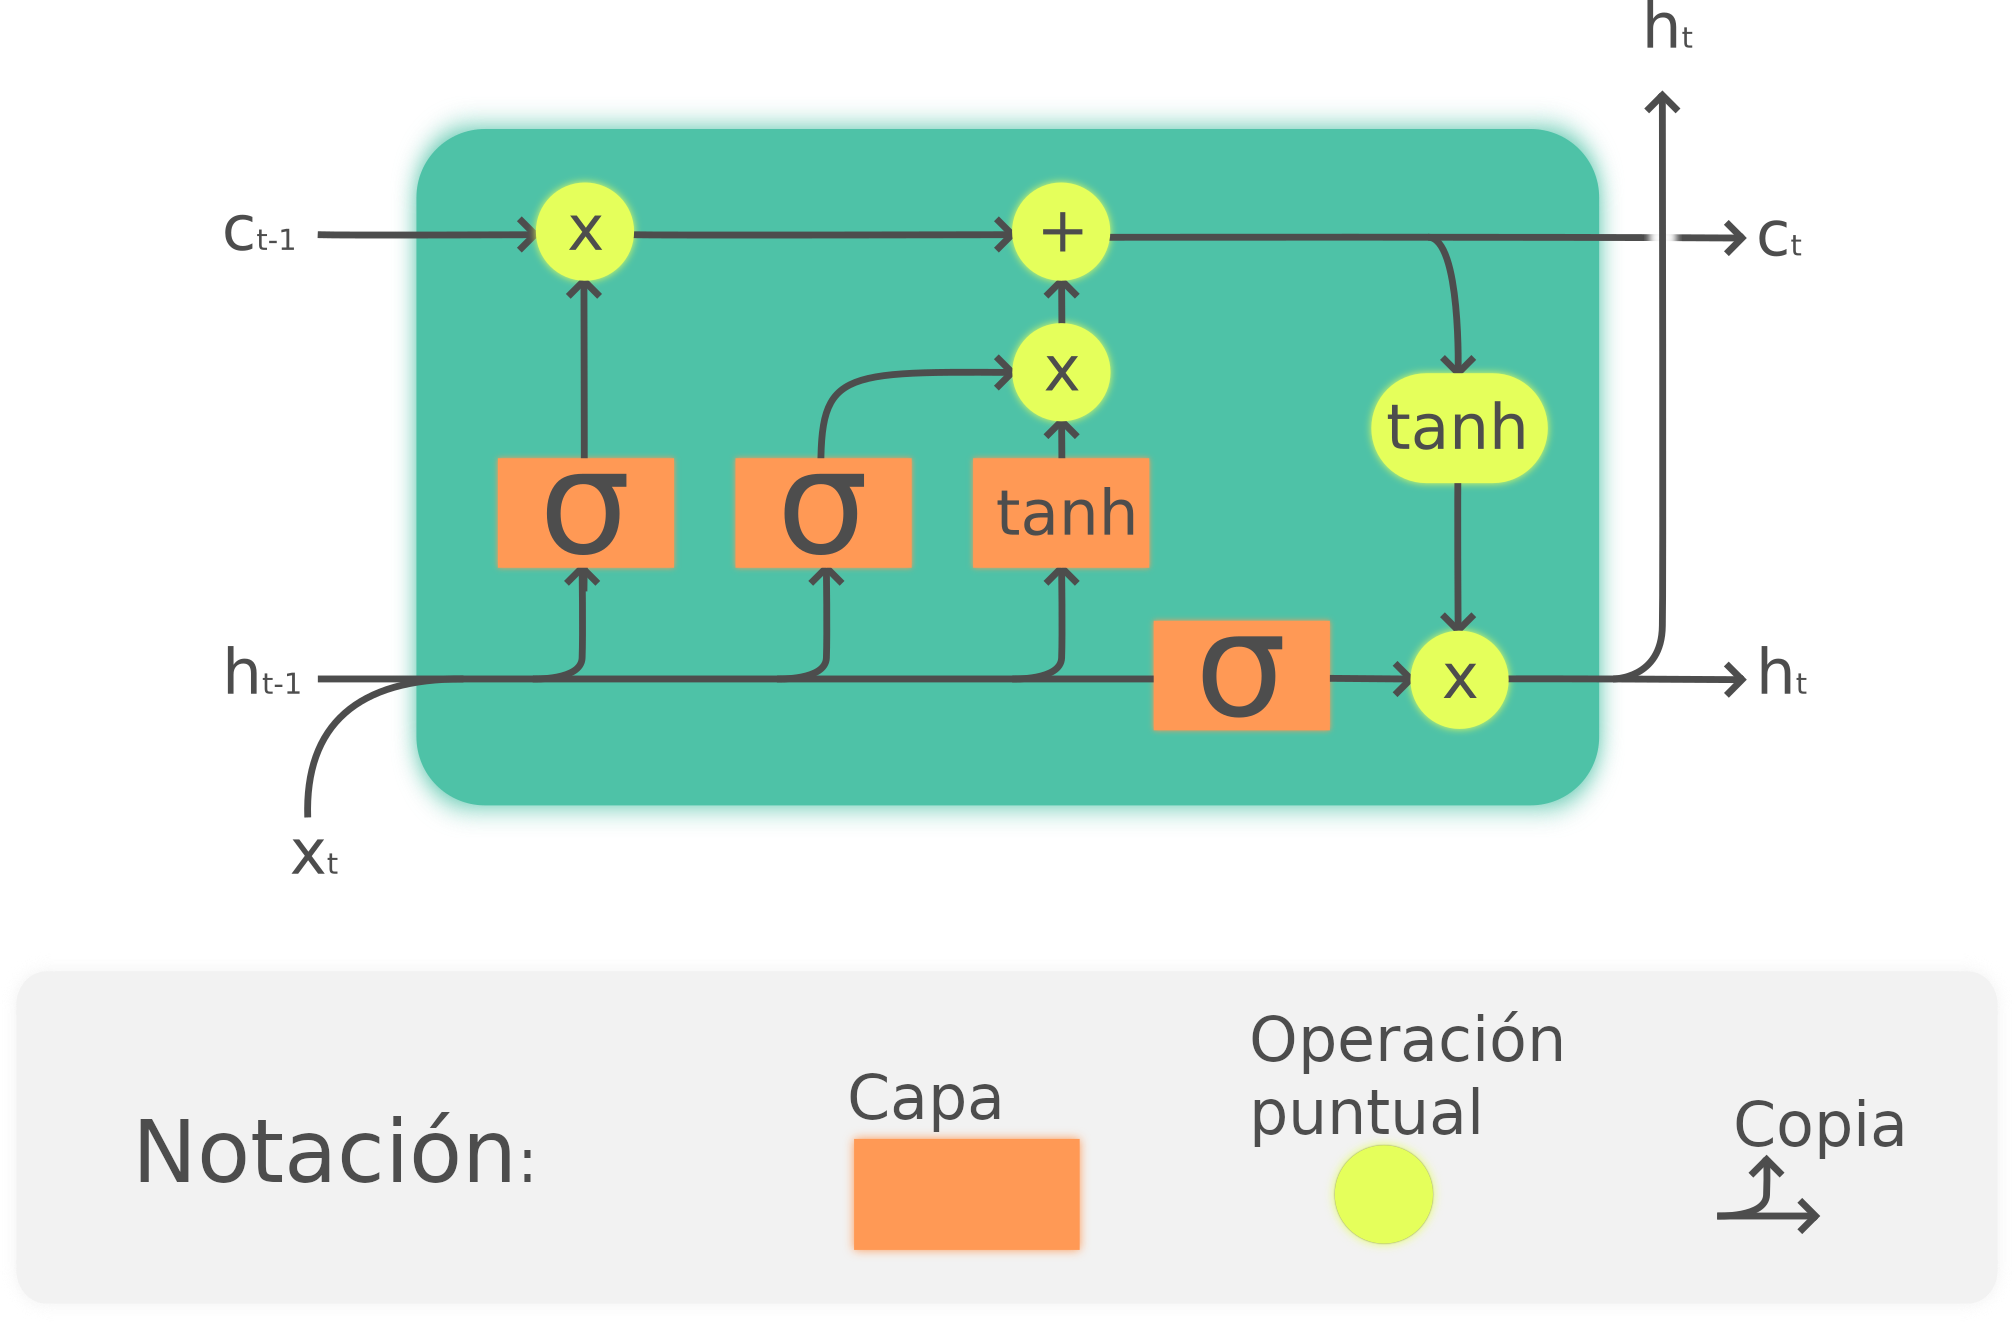
\includegraphics[width=0.7 \textwidth]{sections/figures/LSTM_cell2.png}
\caption{Una celda de LSTM desdoblada sobre el tiempo.} \label{fig:LSTM}
\end{figure}


\subsubsection{Redes Neuronales Convolucionales (CNN)}
Aunque originalmente fueron diseñadas para reconocimiento de caracteres en imágenes, las redes convolucionales han sido empleadas efectivamente para clasificación de textos \citep{kim2014convolutional, zhang2015character, zhang2015sensitivity, conneau2016very}.
En el contexto de clasificación de textos el principal objetivo de este tipo de redes es capturar un contexto local de las palabras en el documento, mediante la aplicación de un conjunto de núcleos de tamaño $d$x$d$. Estas capas de convolución son llamadas mapas de características y pueden ser apiladas para proporcionar múltiples filtros de la entrada. Para reducir la complejidad computacional, las CNNs utilizan una operación llamada pooling la cual reduce el tamaño de la salida de una capa a la siguiente en la red. Existen diferentes técnicas de pooling para reducir la salida y conservar características importantes. El pooling más empleado es el método de max pooling, el cual selecciona el elemento máximo en la ventana de pooling. Para pasar la salida de las capas de pooling, los mapas son \textit{aplanados} en una columna. La capa final en una CNN es típicamente una capa totalmente conectada.


%\subsection{Limitaciones del aprendizaje profundo}
